%LyX 2.0.6 created this file.  For more info, see http://www.lyx.org/.
%Do not edit unless you really know what you are doing.
\documentclass[oneside,english]{amsart}
\usepackage[T1]{fontenc}
\usepackage[latin9]{inputenc}
\usepackage{amsthm}
\usepackage{fullpage}
\usepackage{graphicx}
%\usepackage{enumerate}
\usepackage{float}
\usepackage{amsmath}
\usepackage{url} % click on urls 

\usepackage[parfill]{parskip}
\usepackage{hyperref}
\usepackage{xcolor}

\usepackage{enumitem}

\makeatletter
%%%%%%%%%%%%%%%%%%%%%%%%%%%%%% Textclass specific LaTeX commands.
\numberwithin{equation}{section}
\numberwithin{figure}{section}

\makeatother

\usepackage{babel}
\begin{document}


\hspace{1cm} \\
\vspace{-3.5cm} 

\centerline{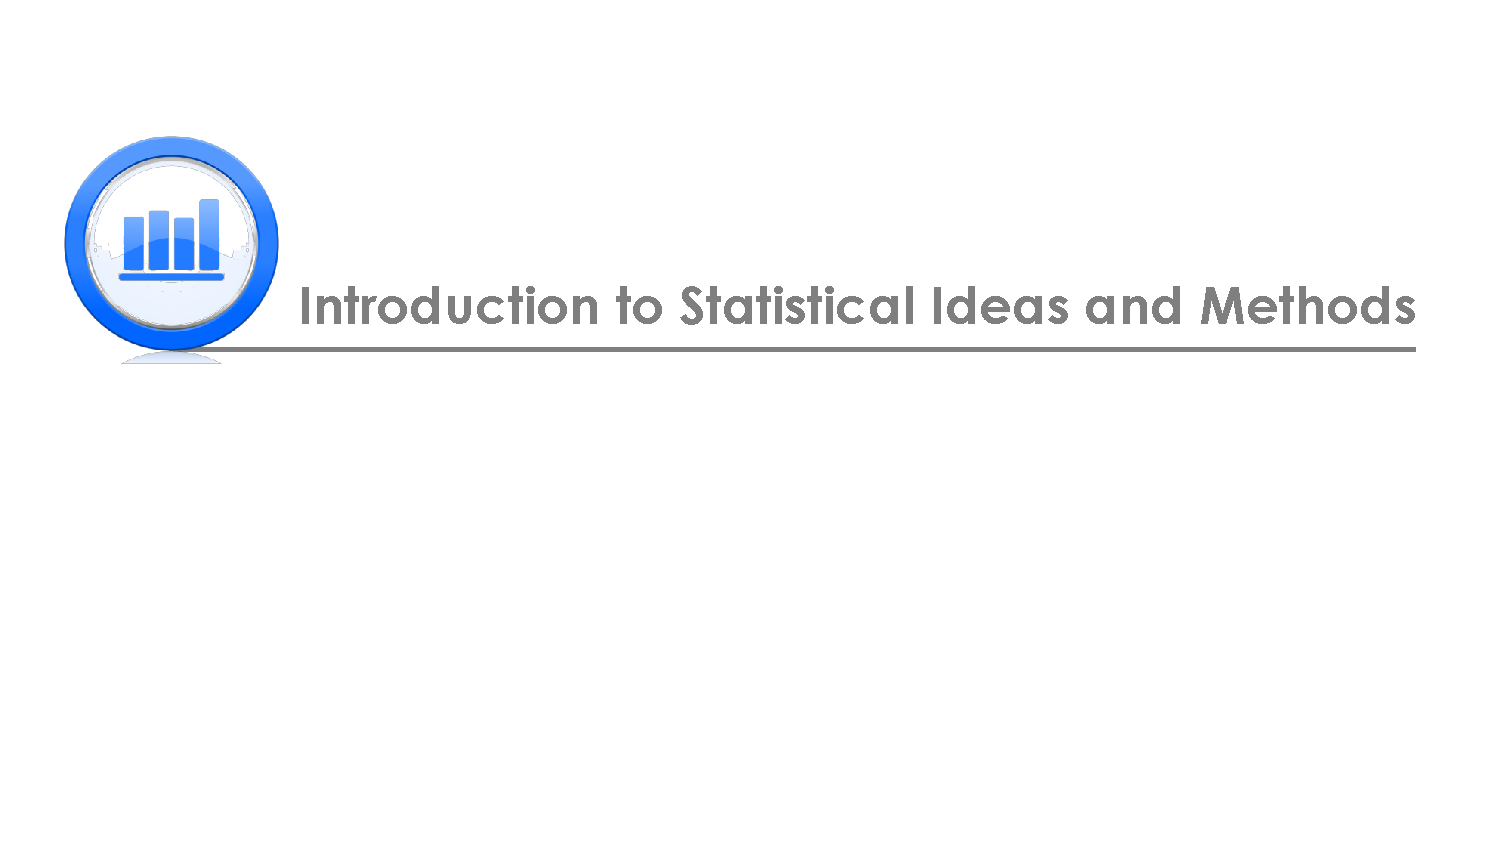
\includegraphics[width=1.1\textwidth]{../../figures/headerfinal.pdf}}

\vspace{.5cm}


%\centerline{{\large{Statistical Tests II: Power App}}} \normalsize  \vspace{.2cm} % Video title
\title{The Effective Use of Statistical Tests: Investigating Power}

\maketitle

The investigating power RShiny application illustrates basic power calculations for hypothesis testing in the proportions setting. 
The application has three main tabs corresponding to single sample testing (with user specified null hypothesis), two sample testing with equal sample sizes and 
two sample testing with unequal sample sizes. Within each tab you may specify all of the values that affect the power of the corresponding test. These are:
\begin{itemize}
\item Sample size: the number of units included in the study.
\item True probability $p$: the actual probability of getting a ``yes'' response on a single trial. For example, the true probability of seeing a heads on a single flip of a coin.
\item Null hypothesis $p_0$ (single sample only): the hypothesized value for the probability of a ``yes'' response that is tested.
\item Alternative hypothesis: two-sided or directed one sided test.
\item Alpha: the significance level of the test.
\end{itemize}
The ``Power'' output gives the computed power for the specified sample size(s). The app also outputs a plot of power against sample size with the other user specified parameters held fixed.
Using the ``Comparison Plots'' subtab it is possible to plot additional power curves corresponding to different testing parameters. In this exercise we'll investigate power for only the single sample case.

Anthropogenic climate change is one of the leading issues the world
faces currently, but it is politically contentious. It is often asserted
by politicians that there is not a scientific consensus on this subject.
This is a serious problem for those who are not experts in the relevant
scientific disciplines and can not assess the evidence directly. It
is natural to ask whether or not there is actually a scientific consensus
on this subject.
\begin{enumerate}
\item How could the question ``is there a consensus about anthropogenic climate change among climate scientists'' be phrased as a hypothesis testing problem?
\vspace{3cm}
\end{enumerate}
Having put this problem in the language of statistical inference we
would like to conduct a study to determine the answer. In this
case the simplest thing to do is randomly survey climate scientists by asking a Yes/No question such as ``Is there adequate evidence to support the conclusion that the climate is changing and that these changes are in large part caused by human activity?'' 
An obvious question to ask is: how many scientists do we need to survey?
The Investigating Power application will help us find the answer to this question. Recall that power is the probability that we will reject the null hypothesis.
\begin{enumerate}[resume]
\item Suppose the null hypothesis is that half of all climate scientists
accept anthropogenic climate change, so $p_{0}=0.5$ and we want to test against alternative hypothesis $p>p_0$.
 If the reality
is that the actual proportion of scientists that accept anthropogenic
climate change is $p=0.80$ and we survey $n=100$ scientists then
what is the power at
the $\alpha=0.05$ level? How does this answer change if the true consesus proportion is only $p=0.6$? What if it's $p=0.7$?
\vspace{3cm}
\end{enumerate}
A more common scenario is that we have a guess for the true proportion
and we'd like to use that guess to estimate how large our survey
needs to be in order to reject the null. For example, suppose we think
that the true proportion of proportion of scientists that accept anthropogenic
climate change is $p=0.97$ (e.g. \url{http://climate.nasa.gov/scientific-consensus/}) and we want to
take a very conservative notion of 'consensus' so we decided to
test
\begin{eqnarray*}
H_{0}:p & = & 0.8\\
H_{A}:p & > & 0.8.
\end{eqnarray*}

\begin{enumerate}[resume]
\item In plain English, what does is the meaning of this hypothesis test?
Do you agree that this is a conservative view of 'consensus'?
\item This hypothesis test actually corresponds to the question ``Is there a consesus amongst climiate changes that anthropogenic climate change \emph{is real}.'' Suppose we wanted to see if there's evidence for a negative consensus: how would the test need to be modified?
\vspace{3cm}
\item What is the smallest number of scientists we should survey in order
to have a probability of at least $0.99$ of rejecting the null hypothesis
with $\alpha=0.01$?
\vspace{3cm}
\item If the true consesus proportion was only $p=0.85$ how many scientists should we survey in order to have a probability of at least $0.99$ of rejecting the null hypothesis
with $\alpha=0.01$? How many do we need to survey if we're content to have at least a  $0.95$ probability of rejecting the null hypothesis at the $\alpha=0.05$ significance level?
\item In plain English, what does $\alpha=0.01$ and $\alpha=0.05$ mean in the previous questions?
\vspace{3cm}
\end{enumerate}
In the example just studied the true proportion was radically different
than the null hypothesis. This is known as a strong effect, and it
has the consequence that the null hypothesis can be rejected with
high probability using relatively small sample sizes. In many situations
the difference between the truth and the null hypothesis is subtler
and it may be necessary to make tradeoffs in the survey. In particular,
because of constraints like budget and ethics it is not always possible
to increase sample size indefinitely in order to increase power.
\begin{enumerate}[resume]
\item For each parameter of the test pick the effect on power of changing each of the values:
\begin{enumerate}
\item Try a smaller and a larger value of sample size.  Increasing sample size \textbf{[increases, decreases, doesn't affect]} the power.
\item Try changing both the true probability and the null hypothesis. For alternative hypothesis $p\neq p_0$, increasing the gap $p-p_0$ \textbf{[increases, decreases, doesn't affect]} the power.
\item Try a smaller and a larger value of $\alpha$.  Increasing sample size \textbf{[increases, decreases, doesn't affect]} the power.
\item Explain why the answers you found make sense.
\vspace{3cm}
\end{enumerate}
\item One possible intuition for hypothesis testing is that $p>0.5$ is
a more specific condition than $p\neq0.5$ so it should always be harder
to establish. That is, we might expect that it's harder to establish that there's a positive consesus rather than merely establishing that there's a consesus in some direction.
Set the null hypothesis to $p_0=0.5$ and the true probability to $p=0.6$
and test this intuition by trying different alternative hypothesis
settings. Is the intuition correct? Explain why the answer you found
makes sense.
\vspace{3cm}
\item Increasing $\alpha$ causes power to increase. It seems we could save
a good deal of money on studies by choosing large $\alpha$ values.
Explain why this might not be a good idea.
\vspace{3cm}
\item How does the shape of the curve of the plot of power vs sample size
change for small effects ($p$ near $p_{0}$) and large effects ($p$
far from $p_{0}$)? What does this suggest about the value of increasing
the study size in each of these cases?
\vspace{3cm}
\item What does the plot of power vs sample size look like when $p=p_{0}$?
How does this change if you vary the value of $\alpha$. Explain why
this makes sense.
\end{enumerate}
\end{document}
